\documentclass{beamer}
%\documentclass[handout]{beamer}
\usepackage[hungarian]{babel}
\uselanguage{hungarian}
\languagepath{hungarian}
\deftranslation[to=hungarian]{Theorem}{T\'etel}
\deftranslation[to=hungarian]{Example}{P\'elda}
\deftranslation[to=hungarian]{Definition}{Defin\'ici\'o}
%\usepackage[magyar]{babel}
\usepackage[utf8]{inputenc}
\usepackage[T1]{fontenc}
\usepackage{beamerthemesplit}
\usepackage{pgf,pgffor,pgfplots}
%\pgfplotsset{compat=1.15}
\usepackage{subfig}
\usepackage{xcolor}
\usepackage{verbatim}
\usepackage{listings}
\usepackage{nccfoots}
\newcommand{\framenote}[1]{%
	\Footnotetext{}{\emph{#1}}% Print footnote text
}

\makeatletter
\let\old@lstKV@SwitchCases\lstKV@SwitchCases
\def\lstKV@SwitchCases#1#2#3{}
\makeatother
\usepackage{lstlinebgrd}
\AtBeginEnvironment{figure}{\setcounter{subfigure}{0}}
\makeatletter
%%%%%%%%%%%%%%%%%%%%%%%%%%%%%%%%%%%%%%%%%%%%%%%%%%%%%%%%%%%%%%%%%%%%%%%%%%%%%%
%
% \btIfInRange{number}{range list}{TRUE}{FALSE}
%
% Test in int number <number> is element of a (comma separated) list of ranges
% (such as: {1,3-5,7,10-12,14}) and processes <TRUE> or <FALSE> respectively

\newcount\bt@rangea
\newcount\bt@rangeb

\newcommand\btIfInRange[2]{%
	\global\let\bt@inrange\@secondoftwo%
	\edef\bt@rangelist{#2}%
	\foreach \range in \bt@rangelist {%
		\afterassignment\bt@getrangeb%
		\bt@rangea=0\range\relax%
		\pgfmathtruncatemacro\result{ ( #1 >= \bt@rangea) && (#1 <= \bt@rangeb) 
		}%
		\ifnum\result=1\relax%
		\breakforeach%
		\global\let\bt@inrange\@firstoftwo%
		\fi%
	}%
	\bt@inrange%
}
\newcommand\bt@getrangeb{%
	\@ifnextchar\relax%
	{\bt@rangeb=\bt@rangea}%
	{\@getrangeb}%
}
\def\@getrangeb-#1\relax{%
	\ifx\relax#1\relax%
	\bt@rangeb=100000%   \maxdimen is too large for pgfmath
	\else%
	\bt@rangeb=#1\relax%
	\fi%
}

%%%%%%%%%%%%%%%%%%%%%%%%%%%%%%%%%%%%%%%%%%%%%%%%%%%%%%%%%%%%%%%%%%%%%%%%%%%%%%
%
% \btLstHL<overlay spec>{range list}
%
% TODO BUG: \btLstHL commands can not yet be accumulated if more than one 
%overlay spec match.
% 
\newcommand<>{\btLstHL}[1]{%
	\only#2{\btIfInRange{\value{lstnumber}}{#1}{\color{orange!30}\def\lst@linebgrdcmd{\color@block}}{\def\lst@linebgrdcmd####1####2####3{}}}%
}%
\makeatother

\usepackage{hyperref}
\hypersetup{
	colorlinks = true,
	linkcolor = blue,
	urlcolor  = blue,
	citecolor = blue,
	linkbordercolor = {white},
}
\usepackage{alltt}
\usepackage{tikz,tkz-euclide}
\usetikzlibrary{trees,calc,patterns,angles,quotes}
\usetikzlibrary{shapes,shapes.geometric,shapes.multipart}
\usetheme{Warsaw}
\institute{Szegedi Tudományegyetem}
\pgfdeclareimage[height=0.55cm]{institution-logo}{../szte_logo}
\logo{\pgfuseimage{institution-logo}}

\title{Algoritmusok és adatszerkezetek II.}
\subtitle{Geometriai algoritmusok}
\date{}

\begin{document}

\maketitle

\begin{frame}{Alapfogalmak}
\begin{definition}
	A $P_3=\begin{bmatrix} x_{3} \\	y_{3} \end{bmatrix}$ pontot 
	$P_1=\begin{bmatrix} 
	x_{1} \\	y_{1} \end{bmatrix}$ és 
	$P_2=\begin{bmatrix} x_{2} \\	y_{2} \end{bmatrix}$ pontok \textbf{konvex 
	kombináció}jának nevezzük, amennyiben $x_3=(1-\alpha) x_1 + \alpha x_2$, 
	valamint $y_3=(1-\alpha) y_1 + \alpha y_2$ teljesül valamely $0 \leq \alpha 
	\leq 1$-ra
\end{definition}
\begin{definition}
	$\overline{P_1P_2}$ szakasz a $P_1$ és $P_2$ pontokból konvex 
	kombinációinak halmaza
\end{definition}
\begin{alertblock}{Megjegyzés}
	Ha a pontok sorrendje is számít, irányított szakaszról beszélünk, és 
	$\overrightarrow{P_1P_2}$ módon jelöljük \\
	$\vec{\mathbf{p}}$-vel $\overrightarrow{OP}$-t, vagyis az $O$ 
	origóból a $P$-be menő irányított szakaszt (vektort) jelöljük
\end{alertblock}
\end{frame}

\begin{frame}{A keresztszorzat}

\begin{block}{$P_1 \times P_2$ keresztszorzata}
	$\det\Bigg(\begin{bmatrix} x_{1} & x_{2} \\	y_1 & y_{2} 
	\end{bmatrix}\Bigg) = x_1y_2-x_2y_1 = P_1 \times P_2 = -P_2 \times P_1$
\end{block}

\begin{block}{Megjegyzés}
	A keresztszorzat valójában háromdimenziós fogalom: egy 
	$\overrightarrow{\mathbf{p_1}}$-re és $\overrightarrow{\mathbf{p_2}}$-re 
	merőleges, velük 
	\href{http://nagysandor.eu/harrisonia/CrossProduct_HU.html}{jobbsodrású 
	rendszert alkotó vektor}, melynek hossza $\lvert x_1 y_2 - x_2 y_1 \rvert$. 
	\\
    \pause Más megfogalmazásban $\overrightarrow{\mathbf{p_1}} \times 
    \overrightarrow{\mathbf{p_2}} = 
    \lVert \overrightarrow{\mathbf{p_1}} \rVert \lVert 
    \overrightarrow{\mathbf{p_2}}\rVert \color{red}{\sin({\theta})} 
    \hat{\mathbf{n}}$, ahol 
    $\theta$ a $\overrightarrow{\mathbf{p_1}}$ és 
    $\overrightarrow{\mathbf{p_2}}$ által bezárt szög, valamint 
    $\hat{\mathbf{n}} 
    \perp \overrightarrow{\mathbf{p_1}}$ és $\hat{\mathbf{n}} \perp 
    \overrightarrow{\mathbf{p_2}}$
\end{block}
\end{frame}

\begin{frame}{Forgásirány}
\begin{block}{Keresztszorzat mint előjeles terület}
	$P_1 \times P_2$ megadja az $O$, $P_1$, $P_2$, $P_1+P_2$ koordinátákkal 
	rendelkező paralelogramma előjeles területét
\end{block}
\begin{columns}
	\begin{column}{.1\linewidth}
		\begin{figure}
			\begin{tikzpicture}
				\draw[<->] (0,0)--(2,0) node[right]{$x$};
				\draw[<->] (0,0)--(0,2) node[above]{$y$};
				\draw node[anchor=east] {O};
				\draw[blue,-stealth](0,0)--(.4,1.2) 
				node[anchor=south]{$P_1$};
				\draw[red,-stealth](0,0)--(1.6,.6) 
					node[anchor=north]{$P_2$};
				\draw[red,dashed](1.6,.6)--(2,1.8);
				\draw[blue,dashed](.4,1.2)--(2,1.8) node[anchor=south]
				{\color{black}$P_1+P_2$};
				%\only<2>{
					\draw[black,-stealth](0.745,0.279)--node[right]{m}(.4,1.2);
					\node at (0.85,0.15) {$P$};
				%}
			\end{tikzpicture}
		\end{figure}
	\end{column} \hfill
	\begin{column}{.6\linewidth}
		\begin{itemize}
			\item $\mathbf{P_1 \times P_2 < 0 \Rightarrow P_1}$\textbf{-ből 
			jobbra fordulva érjük el} $\mathbf{P_2}$\textbf{-t}
			\item $P_1 \times P_2 > 0 \Rightarrow P_1$-ből balra fordulva érjük 
			el $P_2$-t
			\item $P_1 \times P_2 = 0 \Rightarrow P_1$ és $P_2$ kollineáris
		\end{itemize}
	\end{column}
\end{columns}
\end{frame}

\begin{frame}{Merre fordul a következő szakasz?}
\begin{itemize}
	\item $\overline{P_0P_1}$ és $\overline{P_1P_2}$ 
	szakaszokat folyamatosan bejárva merre kell fordulni $P_1$ pontban?
	\item Az előzőekben lényegében az origó viselkedett $P_0$-ként
\end{itemize}

\begin{block}<2>{Ötlet: tegyünk úgy, mintha $P_0$ lenne az origó}
	$(P_1-P_0) 
	\times (P_2-P_0) = \det\Bigg(\begin{bmatrix} x_1 - x_0  & x_2 - x_0 \\	y_1 
	- y_0 & y_2 - 
	y_0 
	\end{bmatrix}\Bigg)$ % = (x_1-x_0)(y_2-y_0)-(x_2-x_0)(y_1-y_0)$
\end{block}

\begin{itemize}
	\item<2> Szemléletesen: $P_1$-ből és $P_2$-ből $P_0$-t kivonva $P_0$ 
	központúvá tesszük a koordinátarendszerünket
\end{itemize}

\end{frame}

\begin{frame}{Szakasz átfogása}

\begin{block}{Átfogó szakasz}
Egy $\overline{P_1P_2}$ szakasz átfog egy egyenest, ha a $P_1$ pont az egyenes
egyik oldalára, $P_2$ pont pedig a másik oldalára esik
\end{block}
\begin{figure}
			\begin{tikzpicture}[scale=.7]
	\tkzInit[xmax=5,ymax=3,xmin=0,ymin=0]
	\tkzAxeXY
	\node (E) at (5.5,2.5) {};
	\node (F) at (-.5,.5) {};	
	\node[outer sep=0pt,circle, fill,inner 
	sep=2pt,label={above:$P_1$}] (C) at (2,3) {};
	\node[outer sep=0pt,circle, fill,inner sep=2pt, 
	label={above:$P_2$}] (D) at (5,1) {};
	
    \draw[dashed,red] (E)--(F);
	\draw[line width=.1em] (C)--(D);
	\end{tikzpicture}
\end{figure}

\begin{block}<2>{Átfedés meglétének eldöntése}
	Egy (kevéssé hatékony) lehetőség, ha az egyenes egyenletét kiszámolva 
	döntünk $P_1$ és $P_2$ relatív helyzetéről \\
	\textbf{Támaszkodjunk helyette a forgásirányokra!}
\end{block}

\end{frame}

\begin{frame}{Egymást metsző szakaszok}
\begin{block}{Szükségesség}
	$\overline{CD}$ úgy metszheti $\overline{AB}$ szakaszt, ha $\overline{CD}$ 
	átfogja az $\overline{AB}$ szakaszra illeszkedő egyenest.
\end{block}

\begin{columns}
	\begin{column}{.5\linewidth}
		\begin{tikzpicture}[scale=.8]
		\tkzInit[xmax=5,ymax=3,xmin=0,ymin=0]
		\tkzAxeXY
		\node[outer sep=0pt,circle, fill,inner 
		sep=2pt,label={above:$A$}] (A) at (1,1) {};
		\node[outer sep=0pt,circle, fill,inner sep=2pt, 
		label={above:$B$}] (B) at (4,2) {};
		\node (E) at (5.5,2.5) {};
		\node (F) at (-.5,.5) {};	
		\node[outer sep=0pt,circle, fill,inner 
		sep=2pt,label={above:$C$}] (C) at (2,3) {};
		\node[outer sep=0pt,circle, fill,inner sep=2pt, 
		label={above:$D$}] (D) at (5,1) {};
		
		\only<2>{\draw[dashed,red] (E)--(F)};
		\draw[line width=.1em] (A)--(B);
		\draw[line width=.1em] (C)--(D);
		\end{tikzpicture}
	\end{column}
	\begin{column}<2>{.5\linewidth}
		\begin{tikzpicture}[scale=.8]
		\tkzInit[xmax=5,ymax=3,xmin=0,ymin=0]
		\tkzAxeXY
		\node[outer sep=0pt,circle, fill,inner 
		sep=2pt,label={above:$A$}] (A) at (1,1) {};
		\node[outer sep=0pt,circle, fill,inner sep=2pt, 
		label={below:$B$}] (B) at (3.25,1.75) {};
		\node (E) at (5.5,2.5) {};
		\node (F) at (-.5,.5) {};	
		\node[outer sep=0pt,circle, fill,inner 
		sep=2pt,label={above:$C$}] (C) at (2,3) {};
		\node[outer sep=0pt,circle, fill,inner sep=2pt, 
		label={above:$D$}] (D) at (5,1) {};
		
		\only<2>{\draw[dashed,red] (E)--(F)};
		\draw[line width=.1em] (A)--(B);
		\draw[line width=.1em] (C)--(D);
		\end{tikzpicture}
	\end{column}
\end{columns}
\end{frame}

\begin{frame}[fragile]{Metszés vizsgálata}
\begin{columns}
	\begin{column}{.6\linewidth}
		\begin{alltt}
			{\scshape{Forgásirány}}(P1, P2, P3) \{
			   return (P2.x-P1.x)*(P3.y-P1.y) - (P3.x-P1.x)*(P2.y-P1.y)
			\} \vfill
			{\scshape{MetszőSzakaszok}}(A, B, C, D) \{
			   d1 = {\scshape{Forgásirány}}(A, B, C)
			   d2 = {\scshape{Forgásirány}}(A, B, D)
			   d3 = {\scshape{Forgásirány}}(C, D, A)
			   d4 = {\scshape{Forgásirány}}(C, D, B)
			   return d1 * d2 < 0 és d3*d4 < 0
			\}
		\end{alltt}
	\end{column}
	\begin{column}<2>{.55\linewidth}
		\vskip 1cm
		Ezzel csak ``valódi'' metszéseket találunk meg, a szakaszra 
		illeszkedő végpontú szakaszt nem kezeltük így
	\end{column}
\end{columns}
\end{frame}

\begin{frame}{Metsző szakaszpár keresése}
\begin{itemize}
	\item Adott szakaszok $n$ elemű halmaza, és tudni szeretnénk, hogy van-e 
	köztük egymást metsző szakaszpár
	\item Nyers erővel $\binom{n}{2}=O(n^2)$
	\item Bizonyos egyszerűsítő feltételezések mellett $O(n\log(n))$ is 
	megoldható
	\begin{itemize}
		\item $y$ tengellyel párhuzamos szakaszokat nem kezelünk
		\item Adott szakaszok között nincs 3 egy pontban metsző
	\end{itemize}
\end{itemize}
\end{frame}

\begin{frame}{Metsző szakaszpár keresése -- söprés}
\begin{block}{Söprés}
	Söprés során egy képzeletbeli függőleges \emph{söprő egyenes} halad át 
	geometriai objektumok halmazán (általában balról jobbra)
\end{block}

\begin{block}{Két szakasz összehasonlítása adott $x$ koordináta mentén}
$s_1$ szakasz fölötte van $s_2$-nek $x$-nél ($s_1 \succ_x s_2$), ha $s_1$  
$y$-koordinátája nagyobb $s_2$ $y$-koordinátájánál adott $x$-koordináta mentén.
\end{block}

\begin{columns}
	\begin{column}{.7\linewidth}
\begin{figure}
	\begin{tikzpicture}[scale=.7]
	\tkzInit[xmax=9,ymax=4,xmin=0,ymin=0]
	%   \tkzGrid
	\tkzAxeXY
	\node[outer sep=0pt,circle, fill,inner 
	sep=1.5pt,label={[fill=white]left:$A$}] (A) at (1,3) {};
	\node[outer sep=0pt,circle, fill,inner sep=1.5pt, 
	label={[fill=white]right:$B$}] (B) at (4,2) {};
	\node[outer sep=0pt,circle, fill,inner 
	sep=1.5pt,label={[fill=white]left:$C$}] (C) at (2,3) {};
	\node[outer sep=0pt,circle, fill,inner sep=1.5pt, 
	label={[fill=white]right:$D$}] (D) at (5,3.2) {};
	\node[outer sep=0pt,circle, fill,inner 
	sep=1.5pt,label={[fill=white]left:$E$}] (E) at (4,1) {};
	\node[outer sep=0pt,circle, fill,inner sep=1.5pt, 
	label={[fill=white]right:$F$}] (F) at (8,4) {};
	\node[outer sep=0pt,circle, fill,inner 
	sep=1.5pt,label={[fill=white]left:$G$}] (G) at (4,4) {};
	\node[outer sep=0pt,circle, fill,inner sep=1.5pt, 
	label={[fill=white]right:$H$}] (H) at (8.5,3) {};
	\node[outer sep=0pt,circle, fill,inner 
	sep=1.5pt,label={[fill=white]left:$I$}] (I) at (5,1) {};
	\node[outer sep=0pt,circle, fill,inner sep=1.5pt, 
	label={[fill=white]right:$J$}] (J) at (7,1) {};
	
	\draw (A)--(B);
	\draw (C)--(D);
	\draw (E)--(F);
	\draw (G)--(H);
	\draw (I)--(J);
	\draw[loosely dotted] (1,0)--(1,4) node[above]{$s_1$};
	\draw[loosely dotted] (2,0)--(2,4) node[above]{$s_2$};
	\draw[loosely dotted] (4,0)--(4,4) node[above]{$s_3$};
	\draw[loosely dotted] (5,0)--(5,4) node[above]{$s_4$};
	\end{tikzpicture}
\end{figure}
	\end{column}
	\begin{column}{.4\linewidth}
		\begin{block}<2>{Példák}
			$\overline{GH} \succ_4 \overline{EF}$, de
			$\overline{EF} \succ_8 \overline{GH}$
		\end{block}
	\end{column}
\end{columns}
\end{frame}

\begin{frame}{Szakaszpár metszése a söprő egyenes szemszögéből}
\begin{itemize}
	\item Bármely adott $x$ értékre a $\succ_x$ reláció az $x$-nél lévő söprő 
	egyenest metsző szakaszok teljes rendezése
	\begin{alertblock}{Kulcsészrevétel}
		Ha $\exists$ egymást metsző szakaszpár $\Rightarrow \exists$ 
		söprő egyenes, mely mentén való rendezés esetén azok egymás után 
		következnek
	\end{alertblock}
	\item A söprő egyenes mozgatása
	\begin{itemize}
		\item Elég a szakaszvégpontokban a be,-és kilépő szakaszok alapján 
		összehasonlításokat végezni
	\end{itemize}
	\item Kétféle adathalmazt kell kezelni a keresés során
	\begin{itemize}
		\item Söprő egyenes állapotleírása
		\item Esetpontok rendezett listája
	\end{itemize}
\end{itemize}
\end{frame}

\begin{frame}{Szakaszpár metszése -- állapotleírás és esetpontok}
	\begin{itemize}
		\item A söprő egyenes állapotleírása a szakaszok adott egyenes menti 
		$\succ$ teljes rendezési reláció szerinti rendezését tartalmazza
		\item A söprő egyenes állapotleírásában változás csak esetpontokban 
		(=szakaszvégpontokban) történik
		\item Esetpontok rendezése
		\begin{itemize}
			\item Kovertikális (azonos $x$-koordinátájú) szakaszvégpontok esetén
			a bal/belépő végpontokat a jobb/kilépő végpontok elé soroljuk
		\end{itemize}
		\item Elegendő azt vizsgálni csupán, hogy a
		\begin{itemize}
			\item belépő szakaszok metszik-e megelőzőjüket/rákövetkezőjüket
			\item kilépő szakaszok megelőzője és rákövetkezője metszi-e egymást
		\end{itemize}
	\end{itemize}
\begin{alertblock}<2>{Fontos}
	A mindenkori állapotleírást kiegyensúlyozott keresőfában tároljuk
\end{alertblock}
\end{frame}

\begin{frame}[fragile]{Metsző szakaszpár keresése}
\begin{alltt}
{\scshape{Van-E-Metsző-Szakaszpár}}(S) \{ // T az állapotleírás fája
  L = S-beli szakaszvégpontok rendezett listája
  for p in L
  do
    if p egy s szakasz bal végpontja \{
      {\scshape{Beszúr}}(T,s)
      if {\scshape{Megelőz}}(T,s) vagy {\scshape{Rákövet}}(T,s) metszi s-et \{
        return {\scshape{Igaz}}
      \}
    \}
    if p egy s szakasz jobb végpontja \{
      if {\scshape{Megelőz}}(T,s) metszi {\scshape{Rákövet}}(T,s)-t \{
        return {\scshape{Igaz}}
      \}
      {\scshape{Töröl}}(T,s)
  return {\scshape{Hamis}}
\}
\end{alltt}
\end{frame}

\begin{frame}{Metsző szakaszpár keresésének futási ideje}
  \begin{itemize}
  	\item Állapotleírás $T$ kiegyensúlyozott fájának létrehozása $O(1)$
  	\item Szakaszvégpontok rendezése $O(n\log{n})$
  	\item \texttt{for} ciklus ''hossza'' legfeljebb $2n=O(n)$
  	\item {\scshape{Megelőz}}, illetve {\scshape{Rákövet}} metódusok 
  	végrehajtása $O(\log{n})$
  	\begin{block}<2>{}
     $\Rightarrow$ Összességében $O(n\log{n})$
  	\end{block}
  \end{itemize}
\end{frame}

\begin{frame}{Konvex burok definíciója}
\begin{block}{Konvex burok}
	Q ponthalmaz konvex burka az a legkisebb P konvex poligon, 
	amelyre Q minden pontja	vagy P határán van, vagy a 
	belsejében.\\
\end{block}
\begin{columns}
	\begin{column}{.5\linewidth}
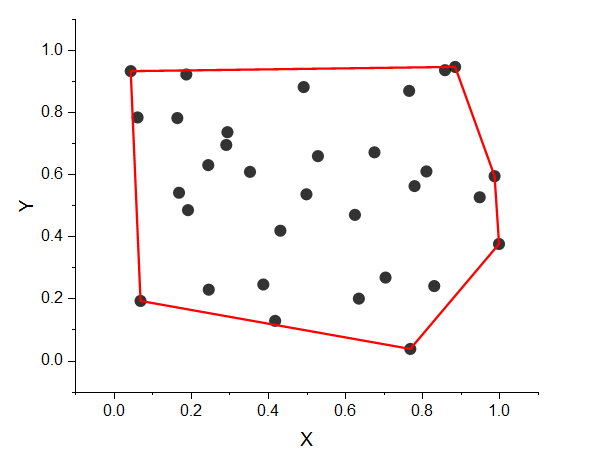
\includegraphics[width=\linewidth]{2D_ConvexHull}
	\end{column}
	\begin{column}{.7\linewidth}
	Q konvex burkát CH(Q)-val jelöljük.\\
    $CH(Q) \subseteq Q$ pontjait $Q$ \textbf{extrém pont}jainak. \\
    Jelöljük a továbbiakban $\lvert Q \rvert$-t $n$-nel.
    
	\end{column}
\end{columns}
\end{frame}

\begin{frame}{CH gyakorlati felhasználása}
\begin{itemize}
	\item Objektumok ütközésének elkerülése: vegyük akadályok 
	koordinátáit, ezek CH-a képezze az elkerülendő régiót
	\item Agglomeratív klaszterezés: gépi tanuló eljárás, melynek célja 
	vektorokkal leírt megfigyelések homogén részsokaságainak kialakítása
\end{itemize}
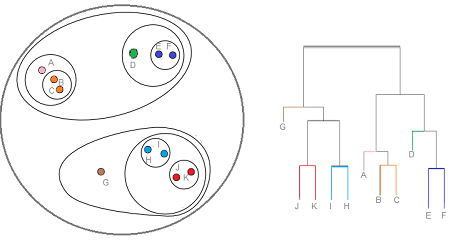
\includegraphics[width=\linewidth]{clustergram}
\end{frame}




\begin{frame}{Konvex burok meghatározásának elvi algoritmusa}
\begin{theorem}
$P$ pont csak abban az esetben extrém pontja $Q$-nak, ha
az a $Q$-ból kialakítható háromszögek mindegyikén kívül esik, vagy annak egy 
csúcsa.
\end{theorem}
\begin{itemize}
	\item Egy csúcs extrém voltának eldöntése $\binom{n-1}{3}=O(n^3)$
	\item Mivel $n$ csúcs van, így az elvi algoritmus $O(n^4)$ futási idejű
\end{itemize}
\end{frame}

\begin{frame}{Konvex burok meghatározása hatékonyan}
\begin{itemize}
	\item Különféle megközelítések léteznek
	\begin{enumerate}
		\item Növekményes módszer: ''balról jobbra'' számítjuk ki a CH-t
		\item Oszd-meg-és-uralkodj: CH számítása a pontok részhalmazára, majd 
		ezek egyesítése
		\item Eltávolító és kereső módszer
	\end{enumerate}
	\item $n$ pont esetében többnyire $O(n \log n)$ futási idejű algoritmusok, 
	de vannak $O(nh)$, illetve $O(n \log h)$ algoritmusok is\footnote{$h$ a 
	CH-ban lévő csúcsok száma}
\begin{block}<2>{Megjegyzés}
	Egy $O(nh)$ algoritmusnak nyilván csak $h < \log{n}$ esetén van haszna
\end{block}
\end{itemize}

\end{frame}

\begin{frame}[fragile]{Konvex burok -- Graham-féle pásztázás}
\begin{alltt}
{\scshape{Graham-pásztázás}}(S) \{
  P0 = minimális x-koordinátájú Q-beli pont (több ilyen
  esetén válasszuk az y-koordináta szerint is minimálisat)
  P = {\scshape{PolárszögSzerintRendez}}(Q)
  S = {\scshape{VermetLétesít}}()
  {\scshape{Verembe}}(P0, S)
  {\scshape{Verembe}}(P1, S)
  {\scshape{Verembe}}(P2, S)
  for i=3 to m \{
    while {\scshape{Legfelső-alatti(S)}}, {\scshape{Legfelső(S)}} és Pi nem 
           fordul balra \{
      {\scshape{Veremből(S)}}
    \}
    {\scshape{Verembe}}(Pi, S)
  \}
  return S
\}
\end{alltt}
\end{frame}

\begin{frame}{Polárszög szerinti rendezés}
\begin{block}{Pontok helyzetének polárkoordinátákkal történő megadása}
$P$ pontot $(x,y)$ koordinátapár helyett egy referenciaponttól vett távolság 
és egy referenciairánnyal bezárt szög párosaként adjuk meg
\end{block}

\begin{itemize}
	\item A refereciaponttól számított $\frac{\Delta y}{\Delta x}$ eltérések 
	szerinti sorrend adja a pontok polárszög szerinti rendezését
	\begin{itemize}
		\item Azonos hányadossal rendelkező pontok közül azt soroljuk előbbre, 
		amelyik a referenciaponthoz közelebb található\footnote{Kivéve, ha 
		$\Delta x=0$, mert akkor a másodlagos rangsorolást fordítva végezzük}
	\end{itemize}
\end{itemize}

\begin{columns}
	\begin{column}{.3\linewidth}
		  \begin{tikzpicture}
		\coordinate (origo) at (0,0);
		
		\fill[black] (origo) circle (0.1);
		\draw[thick,gray,dashed] (0,1) -- ++(0,-3) node (Y) [black,below] {};
		
		\draw[thick] (origo) -- ++(3,-1) coordinate (P);
		\fill (P) circle (0.1);
		
		\pic [draw, ->, "$\theta$"] {angle = Y--origo--P};
		
		\draw[thick] (origo) -- ++(2,0) coordinate (Q);
		\fill (Q) circle (0.1);
		
		\draw[thick] (origo) -- ++(1,1) coordinate (R);
		\fill (R) circle (0.1);
		\end{tikzpicture}
	\end{column} ~
    \begin{column}{0.8\linewidth}
    	\begin{block}{Megjegyzés}
    		A valóságban a vektor hosszának és forgásszögének kiszámítása 
    		költséges és numerikusan sem jó ötlet (\texttt{sqrt} és 
    		szögfüggvény miatt)
    	\end{block}
    \end{column}
\end{columns}
\end{frame}

\begin{frame}[fragile]{Polárszög szerinti rendezés a gyakorlatban}
\begin{itemize}
	\item Numerikus hibák mérséklése és a 0-val való osztás elkerülésére
	\begin{itemize}
		 \item a forgásszöget a pontszorzattal számoljuk
		 \item a vektor hossza helyett a négyzetét számoljuk
		\begin{itemize}
			\item Emlékeztetőül: $\lVert \vec{p} \rVert_2 = \lVert 
			\overrightarrow{OP} \rVert_2 = \sqrt{\sum_{i=1}^{d} P[i]^2}$
		\end{itemize}
	\item Bármilyen összehasonlító rendezést (pl.~gyorsrendezés) tudunk 
használni a forgásirányokra támaszkodva
	\end{itemize}
\end{itemize}

\begin{block}{\texttt{pontok} lista rendezése \texttt{R} referenciapont mentén}
	\begin{alltt}
Collections.sort(pontok, (A, B) -> {
  return (int) Math.signum({\scshape{Forgásirány}}(R, A, B));
});
\end{alltt}
\end{block}
\end{frame}

\begin{frame}{Zárt nem metsző poligon}
\begin{itemize}
	\item A pontokat a polárszöges rendezés sorrendjében 
	összekötve megkapjuk a pontok által alkotott zárt, nem metsző poligont
\end{itemize}

\begin{columns}
	\begin{column}{.8\linewidth}
		\begin{tikzpicture}
		\tkzInit[xmax=7,ymin=0,ymax=4,xmin=0,ymin=0]
		\tkzAxeXY
		\node[outer sep=0pt,circle, fill,inner 
		sep=1.5pt,label={[fill=white]left:$A$}] (A) at (1,1) {};
		\node[outer sep=0pt,circle, fill,inner sep=1.5pt, 
		label={[fill=white]right:$B$}] (B) at (1,3) {};
		\node[outer sep=0pt,circle, fill,inner 
		sep=1.5pt,label={[fill=white]left:$C$}] 
		(C) at (3,2) {};
		\node[outer sep=0pt,circle, fill,inner 
		sep=1.5pt,label={[fill=white]north 
			east:$E$}] 
		(E) at (5,0) {};
		\node[outer sep=0pt,circle, fill,inner sep=1.5pt, 
		label={[fill=white]right:$F$}] (F) at (5,2) {};
		\node[outer sep=0pt,circle, fill,inner 
		sep=1.5pt,label={[fill=white]north:$G$}] 
		(G) at (4,4) {};
		\node[outer sep=0pt,circle, fill,inner sep=1.5pt, 
		label={[fill=white]north:$H$}] (H) at (7,3) {};
		\node[outer sep=0pt,circle, fill,inner sep=1.5pt, 
		label={[fill=white]north:$D$}] (D) at (1,4) {};
		
		\draw (A)--(E);
		\draw (E)--(F);
		\draw (F)--(H);
		\draw (H)--(C);
		\draw (C)--(G);
		\draw (G)--(D);
		\draw (D)--(B);
		\draw (B)--(A);
		\end{tikzpicture}
	\end{column}
	\begin{column}{.2\linewidth}
		\begin{block}{A rendezés}
			\begin{enumerate}
				\item A
				\item E
				\item F
				\item H
				\item C
				\item G
				\item D
				\item B
			\end{enumerate}
		\end{block}
	\end{column}
\end{columns}
\begin{alertblock}<2>{}
	A pontok polárszög szerinti rendezésével nyert sorrendben történő 
összekötése nem feltétlen eredményez konvex poligont
\end{alertblock}
\end{frame}

\begin{frame}{Graham-féle pásztázás példa}
\begin{itemize}
	\item Kezdetben: $S=[A,E,F]$
	\begin{enumerate}
		\item {\scshape{Forgásirány}}(E,F,H), {\scshape{Veremből}}(S), 
		{\scshape{Forgásirány}}(A,E,H), {\scshape{Verembe}}(S, H)
		\item {\scshape{Forgásirány}}(E,H,C), {\scshape{Verembe}}(S, C)
		\item {\scshape{Forgásirány}}(H,C,G), {\scshape{Veremből}}(S), 
		{\scshape{Forgásirány}}(E,H,G), {\scshape{Verembe}}(S, G)
		\item {\scshape{Forgásirány}}(H,G,D), {\scshape{Verembe}}(S,D)
		\item {\scshape{Forgásirány}}(G,D,B), {\scshape{Verembe}}(S,B)
	\end{enumerate}
	\item Végezetül: $S=[A,E,H,G,D,B]$
\end{itemize}
\end{frame}

\begin{frame}{CH meghatározása Jarvis meneteléssel}
\begin{itemize}
	\item Ajándékcsomagolás elvén működik $O(nh)$ időben
	\item Kezdésnek válasszuk ki a legbaloldalibb pontot
	\item Amíg vissza nem érünk a kezdőpontba, válasszuk ki a legutolsónak 
	választott ponttól leginkább balra eső pontot (vagyis azt a pontot, 
	amelytől minden további ponthoz jobbra fordulásra van szükség)
	\item A Jarvis-féle menetelés folyamatosan bővíti CH(Q)-t (egy iterációban 
	$O(n)$ próbát tesz), "vakvágányoktól mentes"
	\begin{itemize}
	\item A Graham-féle pásztázás minden csúcsot potenciálisan CH(Q)-beliként 
	kezel
	\end{itemize}
\end{itemize}
\end{frame}

\begin{frame}{Jarvis menetelése illusztrálva}
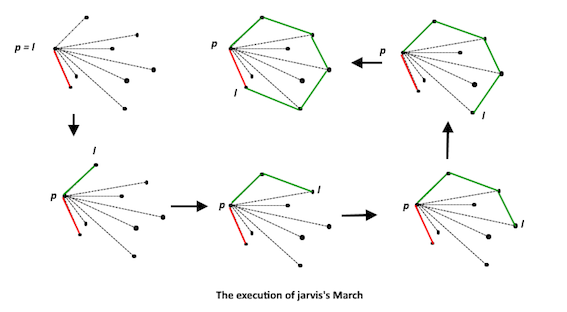
\includegraphics[width=1.1\linewidth]{JarvisAlgorithm}
\end{frame}

\begin{frame}{CH(Q) várható mérete}
\begin{itemize}
	\item Négyzeten/körlapon 2d-ben \textbf{véletlenszerűen} elhelyezkedő 
	ponthalmaznak 
	átlagosan $O(\log{n})$/$O(n^{1/3})$ elemű a CH-ja
\end{itemize}
\begin{columns}
	\begin{column}{0.5\linewidth}
		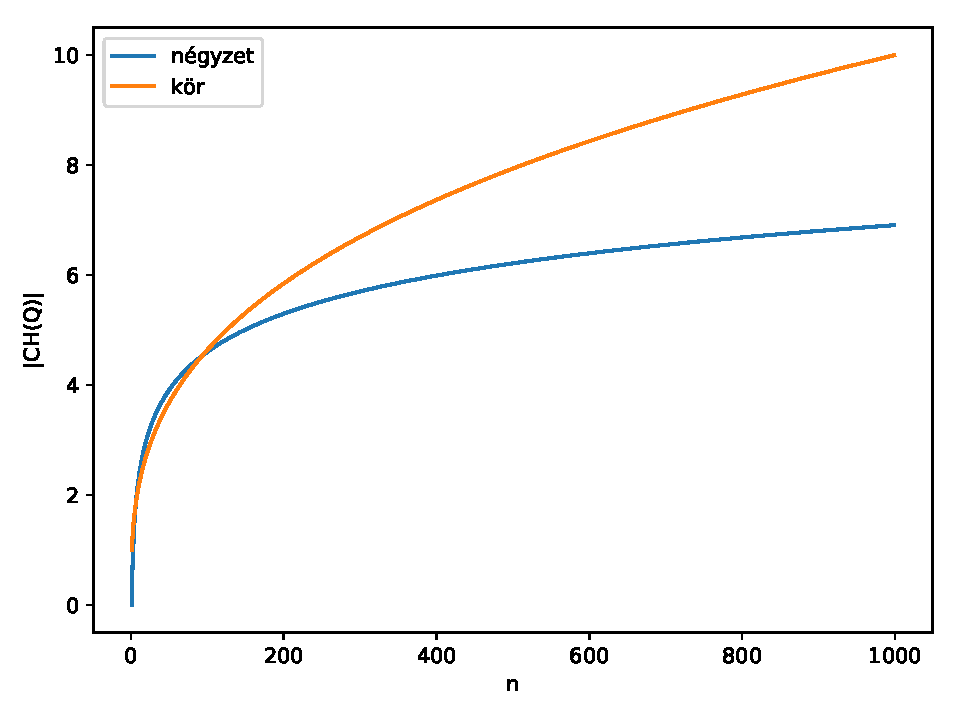
\includegraphics[width=\linewidth]{random_data_ch}
	\end{column}
	\begin{column}{0.5\linewidth}
	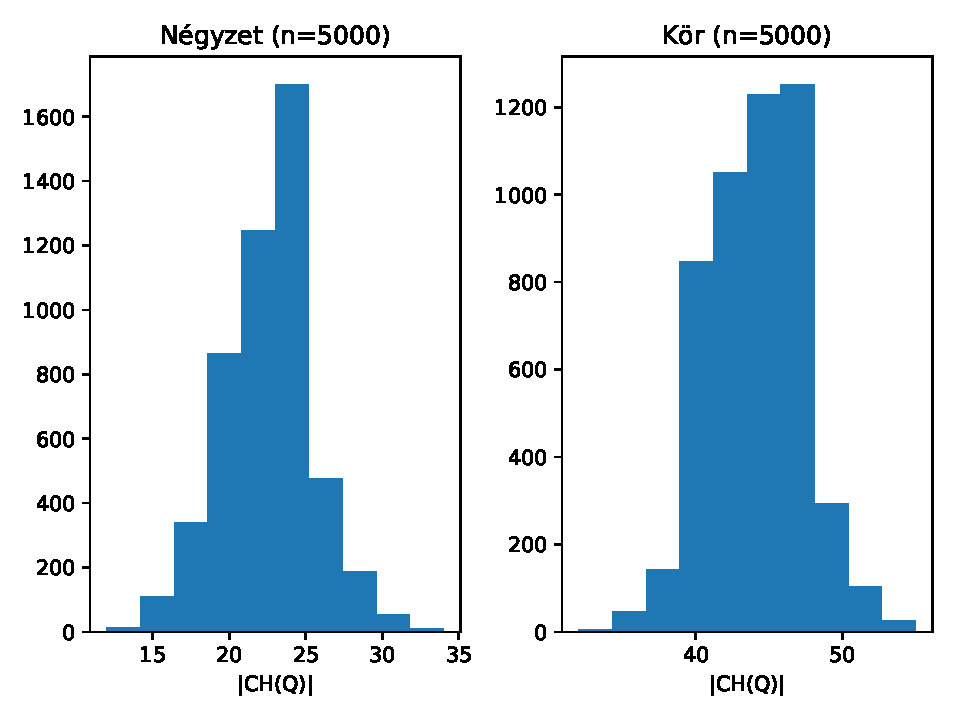
\includegraphics[width=\linewidth]{ch_size_simulation}
\end{column}
\end{columns}
\begin{alertblock}{Ne feledjük!}
	Legrosszabb esetben $CH(Q)=n$ is teljesülhet
\end{alertblock}
\end{frame}

\begin{frame}{Legtávolabbi pontpár megtalálása}
\begin{itemize}
	\item $n$ elemű ponthalmazban találjuk meg azon $(P_i, P_j)$ pontpárt, 
	melyek a legtávolabb fekszenek egymástól
	\begin{itemize}
		\item $P_i$ és $P_j$ pontok távolságát euklideszi értelemben véve 
		$d(P_i, P_j) = \sqrt{(x_i -x_j)^2 + (y_i-y_j)^2}$
	\end{itemize}
	\item Nyers erővel ez is $\binom{n}{2}=O(n^2)$ összehasonlítás lenne
\end{itemize}
\begin{alertblock}{Észrevétel}
A ponthalmaz legtávolabbi pontpárja a CH-on található csúcspárok valamelyike 
kell legyen
\end{alertblock}
\end{frame}

\begin{frame}{A legtávolabbi pontpár a CH-on lesz}
\begin{itemize}
	\item Az észrevétel indirekt módon bizonyítható
	\begin{itemize}
		\item Tegyük föl, hogy $P_i$ és $P_j$ pontok közötti távolság 
		maximális, és $P_i \in CH(Q), P_j \notin CH(Q)$
		\item Vegyünk egy $P_i$ középpontú $\lVert \overline{P_iP_j} \rVert$ 
		sugarú gömböt \\
		$\Rightarrow$ egyetlen $P_k \in Q$ pont sem eshet a 
		gömbön kívül\pause, máskülönben nem $(P_i, P_j)$ alkotná a legtávolabbi 
		pontpárt
		$\Rightarrow P_j \in CH(Q)$, ami viszont ellentmondás
	\end{itemize}
\end{itemize}
\end{frame}

\begin{frame}{Legtávolabbi pontpár megtalálása -- forgatásos söprés}
\begin{itemize}
	\item Átellenes (párhuzamos egyenesekre illeszkedő) csúcsokat keresünk, és 
	ezeket görgetjük végig: $O(h)$
\end{itemize}

\begin{columns}
	\begin{column}{.5\linewidth}
	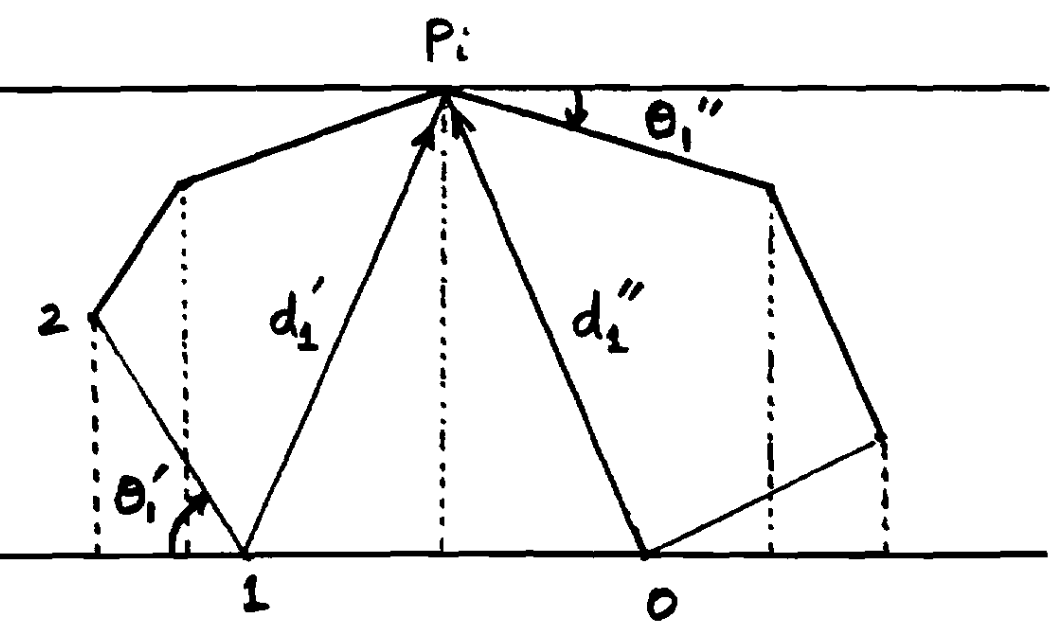
\includegraphics[width=\linewidth]{forgatasos_sopres}
	\end{column} 
	\begin{column}{.5\linewidth}
	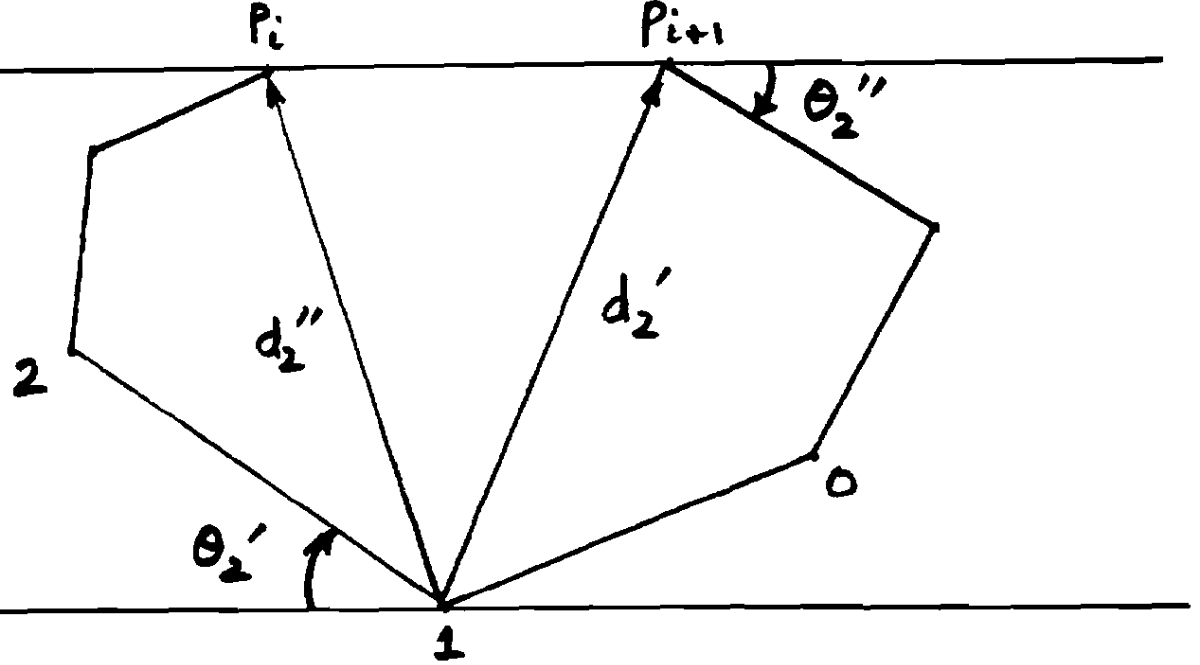
\includegraphics[width=\linewidth]{forgatasos_sopres2}
\end{column}
\end{columns}
\end{frame}

\begin{frame}{Legközelebbi pontpár megtalálása}
\begin{itemize}
	\item Adott $n$ elemű $P$ ponthalmazra mi az a $(P_i, P_j) \in P \times P$ 
	pontpár, ami a legközelebb helyezkedik el egymáshoz?
	\item Nyers erővel szintén $\binom{n}{2}=O(n^2)$
	\item Oszd meg és uralkodj eljárással $O(n\log(n))$ is megoldható
\end{itemize}
\end{frame}

\begin{frame}{Legközelebbi pontpár megtalálása -- oszd meg és uralkodj}
\begin{itemize}
	\item Ha legfeljebb 3 pont maradt, akkor használjuk a nyers erő módszerét
	\item Egyébként hajtsuk végre a következőket
	\begin{itemize}
		\item Vegyük azt az $l$ egyenest, ami két egyenlő részre vágja a 
		pontokat ($P_L$ és $P_R$)
		\item A $P_L$ és $P_R$-beli pontok közül rekurzívan határozzuk meg a
		legközelebbi pontpár közötti távolságot $d=\min(d_L, d_R)$
		\item Döntsük el, hogy találni-e olyan $(P_i, P_j)$ pontpárt, melyre 
		$P_i \in P_L$ és $P_j \in P_R$, továbbá távolságuk $d' < d$
	\end{itemize}
\end{itemize}
\end{frame}

\begin{frame}{Legközelebbi pontpár megtalálása -- illusztráció}
\begin{columns}
	\begin{column}{.5\linewidth}
\begin{figure}
	\centering
	\includegraphics[width=\linewidth]{closepair}
\end{figure}
	\end{column}

	\begin{column}<2>{.6\linewidth}
		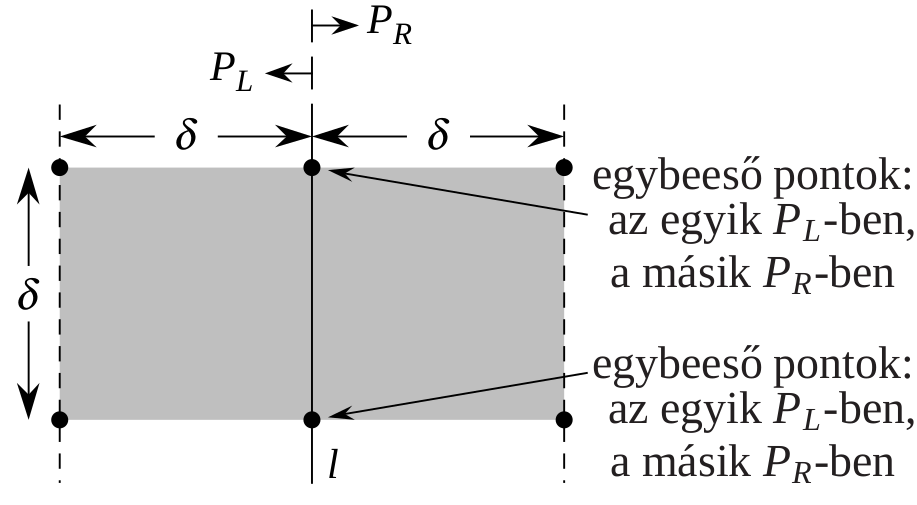
\includegraphics[width=\linewidth]{furthest_points8}
		\begin{block}{Jó hír}
			%$S$ sávon belül sem kell minden pontpárt összehasonlítanunk \\
			Elegendő az $y$ koordináta alapján vett rendezés szerinti 7 
			rákövetkező ponttal összevetni az $S$-beli pontokat
		\end{block}
	\end{column}
\end{columns}
\end{frame}

\begin{frame}{Legközelebbi pontpár megtalálásának hatékonysága}
\begin{itemize}
	\item A pontok $x$ és $y$ koordináta szerinti előrendezésével kezdünk $O(n 
	\log{n})$
	\item A rekurzív lépés során $T(n) = 2*T(\frac{n}{2})+O(n)$ művelet
	\begin{itemize}
		\item Előrendezés nélkül a rekurzív lépés $T(n) = 
		2*T(\frac{n}{2})+O(n \log{n})$ műveletigényű lenne, a teljes eljárás 
		mester módszerrel kapott műveletigénye pedig $O(n \log^2{n})$-re nőne
	\end{itemize}
	\item Az eljárás több szempontból is hasonlít az összefésülő rendezés 
	működéséhez
\end{itemize}
\end{frame}

\begin{frame}{Legközelebbi szomszéd(ok) meghatározása}
\begin{block}{Probléma}
	Adott ponthoz találjuk meg a hozzá legközelebb eső ponto(ka)t
\end{block}

\begin{columns}
	\begin{column}{.6\linewidth}
\begin{block}{Felhasználása}
	Gépi tanulás: k-legközelebbi osztályozó, klaszterező 
	eljárások
\end{block}
	\end{column}
\begin{column}{.3\linewidth}
	\vskip .5cm
	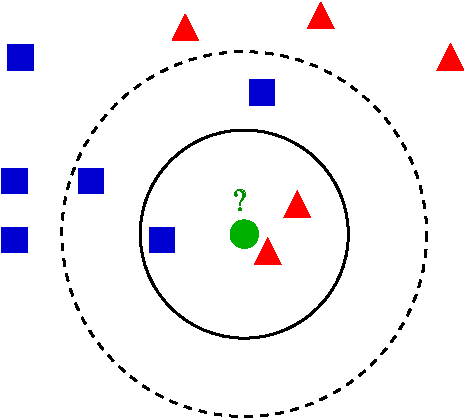
\includegraphics[width=\linewidth]{KnnClassification}
\end{column}
\end{columns}
\end{frame}

\begin{frame}{k-d fák hatékonysága}
\begin{block}{k-d fák}
	$n$ pont esetén a k-d fák fő műveletei átlagos esetben $O(n \log n)$ 
	műveletigényűek
\end{block}

\begin{itemize}
	\item Hatékonysága \href{http://w8r.name/k-d-tree/example/}{statikus 
	ponthalmaz} esetén garantált
	\item Egy k-d fa módosítása (beszúrás/törlés) a kiegyensúlyozottságának 
	megtartása mellett nem triviális
\end{itemize}
\end{frame}

\begin{frame}{k-d fák illusztrációja}
\begin{itemize}
	\item A fa minden szintje a pontok váltakozó koordináták mentén történő 
	megfelezését szolgálják (egyéb stratégiák is léteznek)
	\begin{itemize}
		\item A fa egy csúcsa ossza ketté a részfában található pontokat az 
		adott szintre vonatkozó dimenzió mentén
		\item A fa kiegyensúlyozott lesz, mivel a részfák 
		olyan féltereket definiálnak, amelyeket a mediánok mentén hozunk létre
	\end{itemize}
\end{itemize}
\begin{columns}
	\begin{column}{.55\linewidth}
		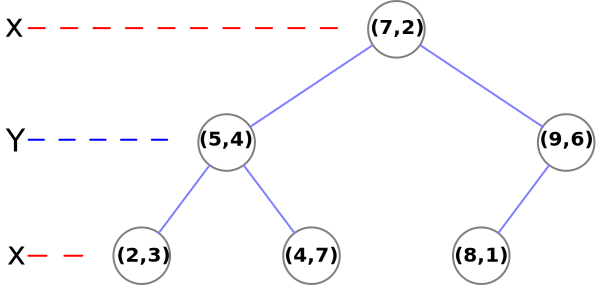
\includegraphics[width=\linewidth]{kd_Tree}
	\end{column}
	\begin{column}{.4\linewidth}
		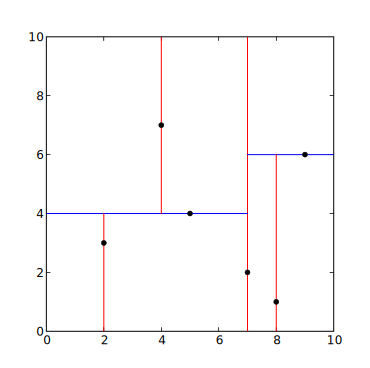
\includegraphics[width=\linewidth]{Kdtree_2d}
	\end{column}
\end{columns}
\end{frame}

\begin{frame}{k-d fában való keresés}
\begin{itemize}
	\item Keressük meg azt a régiót, ahova a lekérdezett pont esik
	\item Nem garantált, hogy a legközelebbi pont ebben a régióban lesz
	\begin{itemize}
	\item<2> Viszont az azon belüli legkisebb távolság alapján sok régió 
	esélytelenné válik a legközelebbi pont tartalmazására nézve
	\end{itemize}
\end{itemize}
\centering
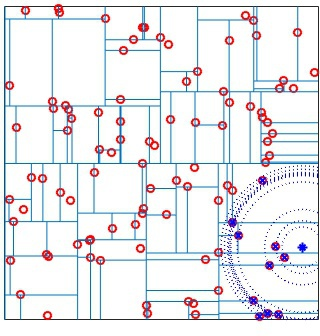
\includegraphics[width=.4\linewidth]{kdtree_uniform_median}
\end{frame}

\begin{frame}{Összefoglalás}
\begin{itemize}
	\item A geometriai algoritmusok számos gyakorlati probléma (pl.~gépi 
	tanulás) megoldása során felmerülnek
	\item A numerikus hibák (egy része) kiküszöbölhető {\scshape{ForgásIrány}} 
	használatával
	\item Nagy méretű inputok esetén fontos, hogy a négyzetes (vagy annál is 
	rosszabb) futási idejű algoritmusoknál hatékonyabbakat használjunk
\end{itemize}
\end{frame}

\end{document}